\documentclass[10pt,twoside]{article}
\usepackage[utf8]{inputenc}
\usepackage{amsmath}
\usepackage{amsfonts}
\usepackage{amssymb}
\usepackage[spanish,es-noshorthands]{babel}
\usepackage[T1]{fontenc}
\usepackage{lmodern}
\usepackage{graphicx,hyperref}
\usepackage{multirow} 
\usepackage{tikz,pgf}
\usepackage{multicol}
\usepackage{subfig}
\usepackage[papersize={6.5in,8.5in},width=5.5in,height=7in]{geometry}
\usepackage{fancyhdr}
\pagestyle{fancy}
\fancyhead[LE]{
\includegraphics[height=12pt]{Images/logo-colegio.png} Aritm\'etica $6^{\circ}$}
\fancyhead[RE]{}
\fancyhead[RO]{\textit{Germ\'an Avenda\~no Ram\'irez, Lic. U.D., M.Sc. U.N.}}
\fancyhead[LO]{}

\author{Germ\'an Avenda\~no Ram\'irez, Lic. U.D., M.Sc. U.N.}
\title{\begin{minipage}{.2\textwidth}

\includegraphics[height=1.75cm]{Images/logo-colegio.png}\end{minipage}
\begin{minipage}{.55\textwidth}
\begin{center}
Taller 07, Multiplicación en $\mathbb{N}$ \\
Aritm\'etica $6^{\circ}$
\end{center}
\end{minipage}\hfill
\begin{minipage}{.2\textwidth}

\includegraphics[height=1.75cm]{Images/logo-sed.png} 
\end{minipage}}
\date{}
\begin{document}
\maketitle
Nombre: \hrulefill Curso: \underline{\hspace*{44pt}} Fecha: \underline{\hspace*{2.5cm}}
\section*{Multiplicaci\'on en $\mathbb{N}$}
\subsection*{Acitividad 1}
Realice en forma individual en su cuaderno lo siguiente:
\begin{itemize}
 \item Tome una hoja de papel. D\'oblela de manera que queden, bien 4 filas y 8 columnas o bien, 8 filas y 4 columnas as\'i:
\begin{center}
\begin{tikzpicture}
\draw[help lines](0,0)grid(8,4);
\node[above] at (0.5,4){Columna 1};
\node[left]at(0,3.5){Fila 1};
\end{tikzpicture}
\end{center}
\item Responda las siguientes preguntas:
\begin{itemize}
 \item ?`En cu\'antas partes queda dividido el papel?
\item ?`Cu\'antos cuadrados tiene cada columna?
\item ?`Cu\'antos cuadrados tiene cada fila?
\item ?`Cu\'anto es 8 veces 4?, es decir, $4+4+4+4+4+4+4+4$
\item ?`Cu\'anto es 4 veces 8?, es decir, $8+8+8+8$.
\item ?`C\'omo se escribe abreviadamente 4 veces 8?, ?`8 veces 4?
\item ?`Qu\'e resultado se obtiene?
\end{itemize}
\item Recuerda:
\end{itemize}
La operación, que es una suma abreviada de sumandos iguales, se llama MULTIPLICACIÓN.
La multiplicación entre dos números naturales $a$ y $b$, se simboliza así:
\[a\cdot b \qquad \text{ó} \qquad a\times b, \qquad \mbox{8 veces 4}=8\cdot 4=8\times 4=4+4+4+4+4+4+4+4=32\]
El punto $\cdot$ y el signo $\times$ indican multiplicación. Cada término que interviene en la
operación se llama FACTOR. El número que se repite se llama MULTIPLICANDO y
el número de veces que el sumando se repite se llama MULTIPLICADOR
\begin{center}
\begin{tabular}{ccccc}
8 & $\times$ & 4 & = & 32 \\ 
Multiplicando &  & Multiplicador &  & Producto \\ 
\multicolumn{3}{c}{Factores}   &  &  \\ 
\end{tabular} 
\end{center}
\section*{Apliquemos las propiedades de la multiplicaci\'{o}n}
\subsection*{Actividad 2}
realizamos las siguientes operaciones y sacamos conclusiones.
\begin{itemize}
\item Respondamos en el cuaderno:
\begin{center}
\begin{tabular}{ll}
\multirow{2}{*}{\fbox{$2\times5=10$}}  & ¿Qué clase de números son el 2 y el 5? \\ 
 & ¿Qué clase de número es el 10? \\ 
\end{tabular} 
\end{center}
\begin{center}
\begin{tabular}{ll}
\multirow{2}{*}{\fbox{$3\times 4=12$}} & ¿Qué clase de números son el 3 y el 4? \\ 
 & ¿Qué clase de número es el 12? \\ 
\end{tabular} 
\end{center}
¿Qué clase de número es el producto de dos números naturales?
\item En el cuaderno realizamos las siguientes multiplicaciones:
\begin{itemize}
\begin{multicols}{2}
\item \begin{tabular}{|c|}
\hline 
$8\times 4=$? \\ 
\hline 
$4\times 8=$? \\ 
\hline 
\end{tabular} 
\item 
\begin{tabular}{|c|}
\hline 
$3\times 7=$? \\ 
\hline 
$7\times 3=$? \\ 
\hline 
\end{tabular}
\item
\begin{tabular}{|c|}
\hline 
$9\times 4=$? \\ 
\hline 
$4\times 9=$? \\ 
\hline 
\end{tabular}
\item 
\begin{tabular}{|c|}
\hline 
$5\times 1=$? \\ 
\hline 
$1\times 5=$? \\ 
\hline 
\end{tabular}  
\end{multicols}
¿Qué podemos concluir?
\end{itemize}
\item En el cuaderno realizamos las siguientes multiplicaciones:
\begin{itemize}
\begin{multicols}{2}
\item 
\begin{tabular}{|c|}
\hline 
$(4\times 2)\times 3=$? \\ 
\hline 
$4\times (2\times 3)=$? \\ 
\hline 
\end{tabular}
\item 
\begin{tabular}{|c|}
\hline 
$(3\times 2)\times 5=$? \\ 
\hline 
$3\times (2\times 5)=$? \\ 
\hline 
\end{tabular} 
\item 
\begin{tabular}{|c|}
\hline 
$(6\times 2)\times 3=$? \\ 
\hline 
$6\times (2\times 3)=$? \\ 
\hline 
\end{tabular} 
\item
\begin{tabular}{|c|}
\hline 
$(3\times 4)\times 3=$? \\ 
\hline 
$3\times (4\times 3)=$? \\ 
\hline 
\end{tabular} 
\end{multicols}
\end{itemize}
¿Qué conclusiones podemos sacar?
\item En el cuaderno. Contemos los puntos.

\begin{minipage}{.5\textwidth}
\begin{tikzpicture}
\draw[help lines] (0,0) grid (6,1);
\filldraw (.5,.5) circle(.5ex) (1.5,.5) circle (.5ex) (2.5,.5)circle(.5ex) (3.5,.5)circle(.5ex) (4.5,.5)circle(.5ex) (5.5,.5)circle(.5ex);
\end{tikzpicture}
\end{minipage}\hfill
\begin{minipage}{.4\textwidth}
6 veces 1 = 6 \\$1+1+1+1+1+1=6\times 1=6$
\end{minipage}

\begin{minipage}{.45\textwidth}
Una vez seis\\
$1\times 6=$?
\end{minipage}
\begin{minipage}{.3\textwidth}
\begin{tikzpicture}
\draw (0,0) rectangle (1,3);
\filldraw (.5,.25)circle(.5ex) (.5,.75)circle(.5ex) (.5,1.25)circle(.5ex) (.5,1.75)circle(.5ex) (.5,2.25)circle(.5ex) (.5,2.75)circle(.5ex);
\end{tikzpicture}
\end{minipage}
\item ¿Qué conclusión podemos sacar?
\end{itemize}
¿Cuánto es

\begin{minipage}{.6\textwidth}
\begin{tabbing}
\hspace{2.5cm}\=\hspace{2.5cm}\=\kill
 $6\times 1=$? \> $7\times 1=$? \> $4\times 1=$?\\
 $1\times 6=$? \> $1\times 7=$? \> $1\times 4=$?
\end{tabbing} 
\end{minipage}\hfill
\begin{minipage}{.35\textwidth}
¿Qué pasa cuando uno de los
factores es 1?
\end{minipage}
\begin{itemize}
\item En el cuaderno realicemos las siguientes operaciones y comparemos los resultados de las dos columnas:

\begin{tabbing}
\hspace{3cm}\=\kill
$2\times (3+5)$ \> $(2\times 3)+(2\times 5)$ \\ 
$3\times (7+2)$ \> $(3\times 7)+(3\times 2)$ \\ 
$4\times (2+6)$ \> $(4\times 2)+(4\times 6)$ 
\end{tabbing}
¿Qué conclusión podemos sacar?
\item Representemos gráficamente en una cuadrícula en la cual el primer natural indica las filas:
\begin{enumerate}
\begin{multicols}{2}
\item[a)] $2\times (3+4)$
\item[b)] $(2\times 3)+(2\times 4)$
\end{multicols}
\end{enumerate}
\end{itemize}
Comparemos los resultados: ¿Qué conclusión sacamos?
\section*{Concluyamos}
La multiplicación entre números naturales cumple las siguientes propiedades:
\begin{enumerate}
\item La multiplicación de dos números naturales es otro número natural.\\
  Propiedad CLAUSURATIVA.
\item El orden de los factores no altera el producto.\\Propiedad CONMUTATIVA.
\item Para multiplicar tres factores podemos agruparlos de diferentes formas y
  efectuar los productos parciales sin que el producto final varíe.\\Propiedad
  ASOCIATIVA.
\item La multiplicación de cualquier número natural por 1, da como resultado el
    mismo número natural.\\Propiedad MODULATIVA. (El módulo del producto
     es el 1).
\item El producto de un número natural por una adición de dos números naturales es igual al producto de dicho número por cada uno de los sumandos.\\Propiedad DISTRIBUTIVA.
\end{enumerate}
Complete el siguiente sudoku. Recuerde que en cada cuadrado $3\times 3$, en cada fila de y en cada columna deben estar los números del 1 al 9 sin repetir n\'{u}mero.
\begin{center}
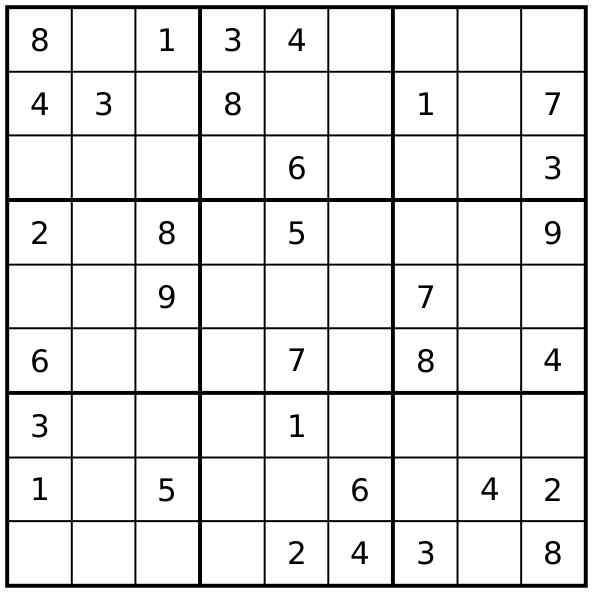
\includegraphics[scale=.35]{Images/sudoku01.png} 
\end{center}
\end{document}
